\section{Evaluation Environment}
\label{sec:testingEnv}

%% 
%% Leave first page empty
\thispagestyle{empty}

We have set up a testing environment to help us run tests for WebRTC. Figure~\ref{fig:evaluation_arch} describes the functional blocks used for the simple video call.

 \begin{figure}[h]
  \centering
    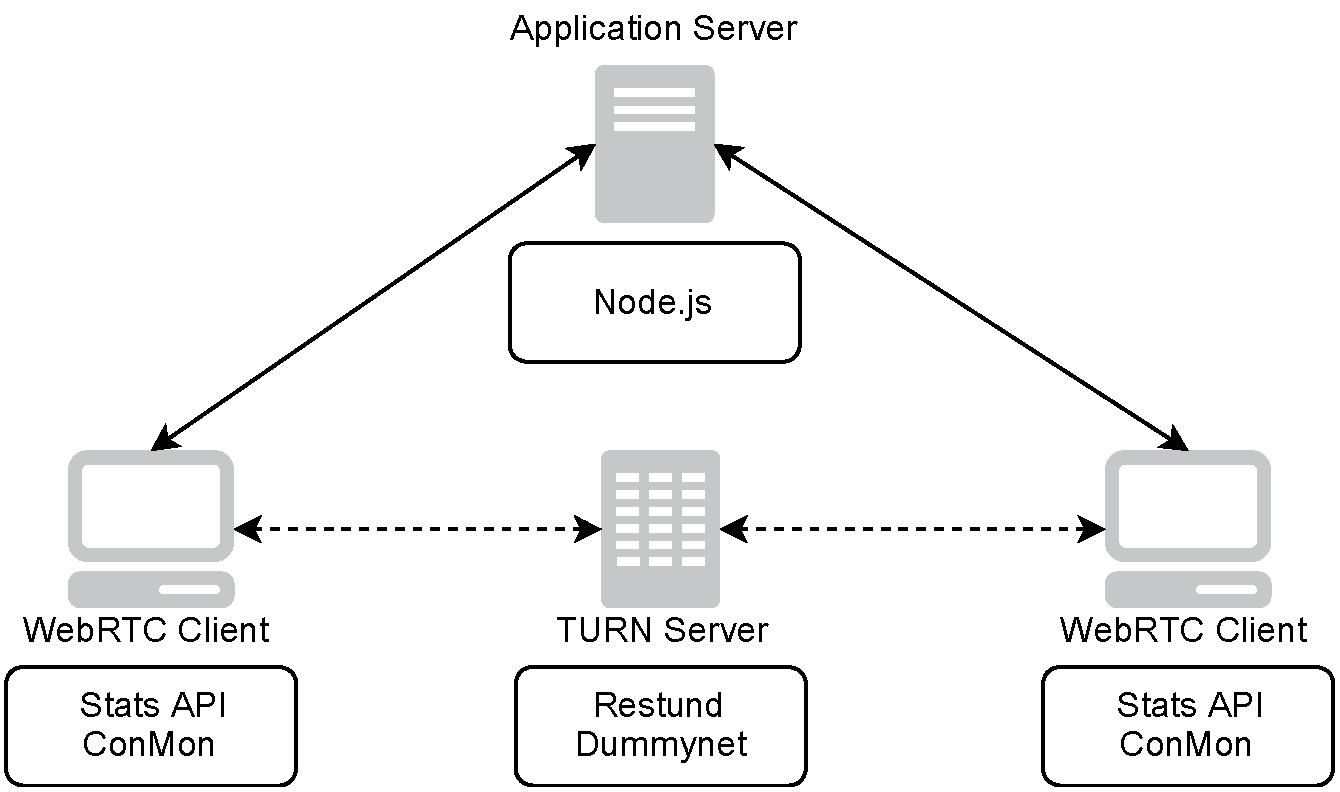
\includegraphics[width=1\textwidth]{./figures/evaluation_arch.pdf}
      \caption[Description of testing environment topology]{Description of testing environment topology.}
	\label{fig:evaluation_arch}
\end{figure}

\subsection{WebRTC client}

WebRTC clients are virtual machines that run a lightweight version of Ubuntu (Lubuntu) with 2GB of RAM and one CPU. This light version avoids the usage of 3D acceleration helping us to get better results in performance than compared with other distributions. 

Clients will be running Chrome Dev version 27.01453.12 as WebRTC capable browser. To avoid modified results due to a bug in the {\it Pulse Audio} module of Ubuntu that controls audio input in WebRTC calls will be done with only video, the amount of audio transferred due to the echo cancelation systems can be neglicted.

\subsubsection{Connection Monitor}

Connection Monitor ({\it ConMon}) is a command line utility that relies on the transport layer and uses TCPDUMP to sniff all the packets that to go a certain interface and port~\cite{singhConMon}. This application is designed to specifically detect and capture RTP/UDP packets, relies on {\it libcap} for the capture in the network layer. This software detects and saves the header but discards the payload of the packet keeping the information we need for calculating our KPIs.

Typically we will run the PeerConnections between two devices and start capturing those packets by using {\it ConMon}. The PeerConnection will carry real data so the environment for testing will be a precise approach to a real scenario of WebRTC usage.

{\it ConMon} captures will be saved into different files and allow us to plot every stream bandwidth and calculate other parameters such as delay by using some parsing, this will allow us to compare how precise are both way of analyzing WebRTC as {\it ConMon} is working directly over the incoming interface and avoids all the processing that the browser is doing to send the stats to the JavaScript layer. Figure~\ref{fig:onetooneWifiRTCConMon} represents one video stream from the same call as Figure~\ref{fig:onetooneWifiRTC} and~\ref{fig:onetooneWifiRTCVideoStreams} but captured from the {\it ConMon} application.

 \begin{figure}[h]
  \centering
    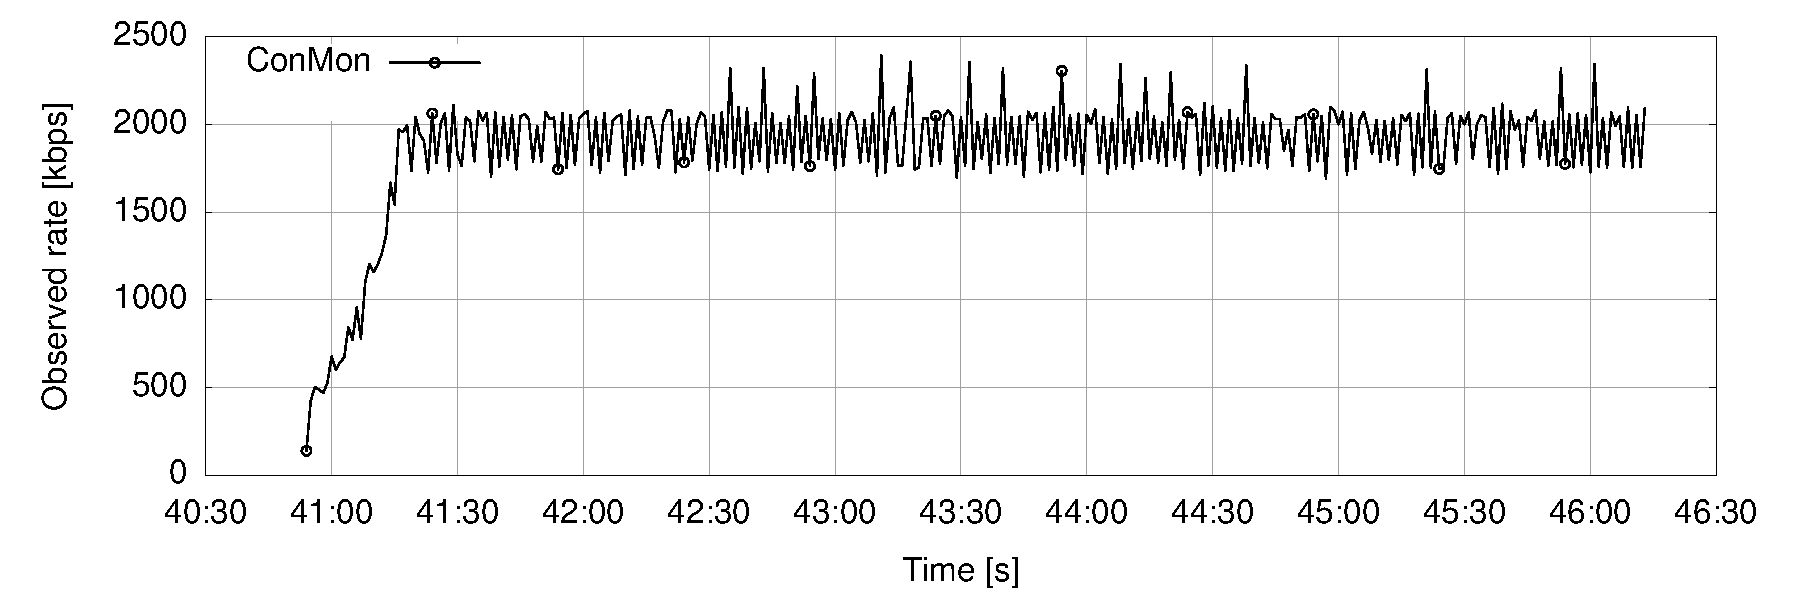
\includegraphics[width=1\textwidth]{./figures/onetooneWiFiConMon.pdf}
      \caption[Point-to-point WebRTC video stream throughput graph using ConMon over public WiFi]{Point-to-point WebRTC video stream throughput graph using ConMon over public WiFi.}
	\label{fig:onetooneWifiRTCConMon}
\end{figure}

The capture from {\it ConMon} will be very accurate capturing all the packets that go through the interface, dumping the values into the output file, this data will then be processed and averaged for every second prior plotting. This processing will lead to some fluctuations on the graph that distort the reality.

\subsubsection{Stats API}

WebRTC carries a subsection of methods to help developers to access the lower layer network information, this methods return all different types of statistics and performance indicators that we will be using to build our own JavaScript Stats API. When using those statistics we will measure all the congestion KPIs to analyze them.

The method used is the RTCStatsCallback returns a dictionary object (JSON) that has be parsed and manipulated to get the correct indicators, this object returns as many streams as available in a PeerConnection, usually audio and video. This data is provided by the lower layers of the network channel using the RTCP packets that come multiplexed in the RTP stream~\cite{rtpusageIETF}.

The Stats API is the way that WebRTC allows the developer to access different metrics, as this is still in an ongoing discussion the stats report object has not been totally defined and can slightly change, the methods used by the Stats API are available on the W3C editors draft ~\cite{editorWebRTCdraft}. 

We have built a JavaScript tool that uses those stats from the browser to calculate the RTT, throughput and loss rate for the different streams that are being received. Those stats can later be saved into a file or sent as a JSON object to a centralized monitoring system. Our JavaScript grabs any PeerConnection passed through the variable and starts looping an iteration to collect those stats and either plot them or save them into an array for post-processing. 

Figure~\ref{fig:onetooneWifiRTC} shows an example capture of a call between two browsers in two different machines, Mac and Ubuntu, the call was made over Wifi open network with no firewall in the middle but with real traffic. The measures are directly obtained from the Stats API JS file we have built and post-processed using {\it gnuplot}.

 \begin{figure}[h]
  \centering
    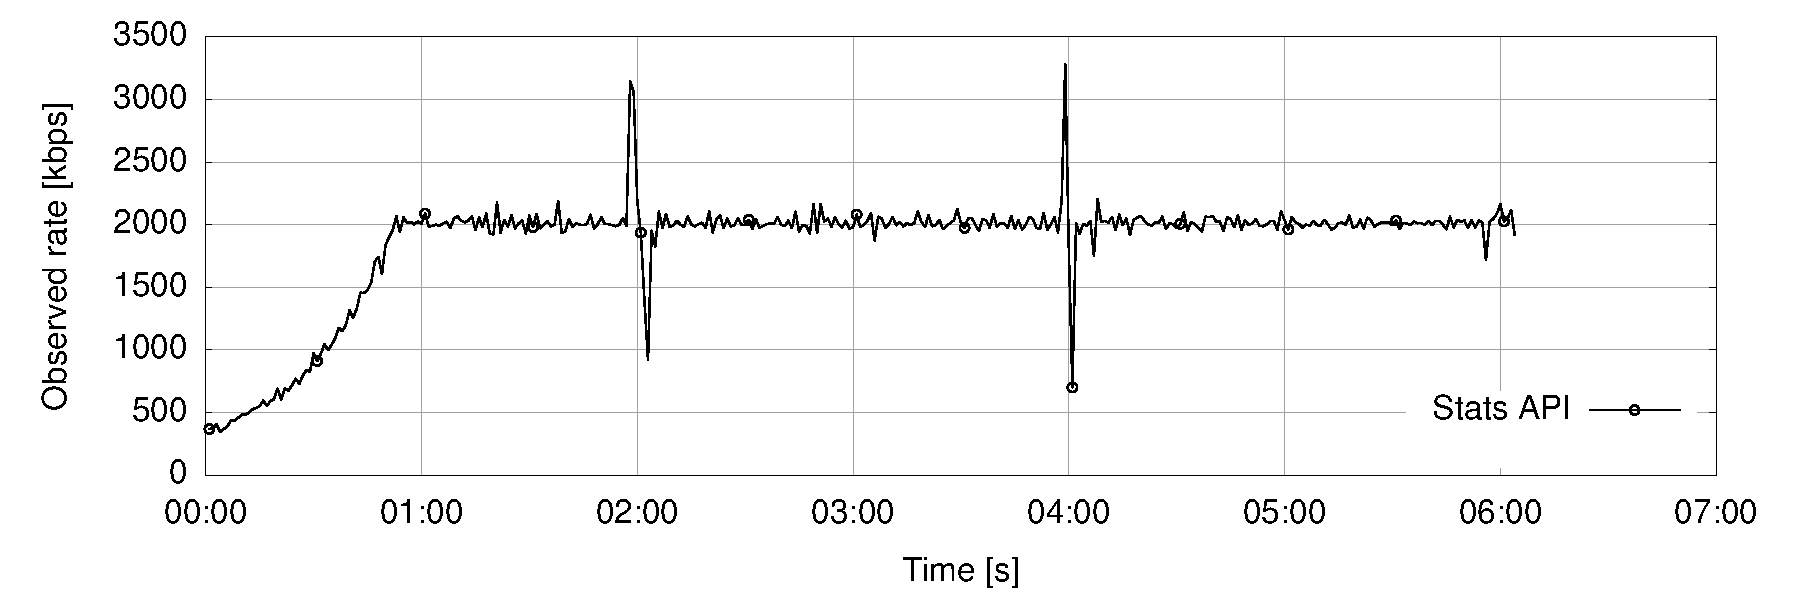
\includegraphics[width=1\textwidth]{./figures/onetooneWifiStatsRTC.pdf}
      \caption[Point-to-point WebRTC video call total throughput graph using Stats API over public WiFi]{Point-to-point WebRTC video call total throughput graph using Stats API over public WiFi.}
	\label{fig:onetooneWifiRTC}
\end{figure}

The previous Figure~\ref{fig:onetooneWifiRTC} considers the global bandwidth of the call, this means that the input/output video and audio are measured together to check how much bandwidth is being consumed over the duration of the call, as it is using RTCP packets for the metrics it takes a while to reach the average rate value. We can then plot all the different streams together to get an idea of how much bandwidth is consuming every PeerConnection.

% \begin{figure}[h]
%  \centering
%    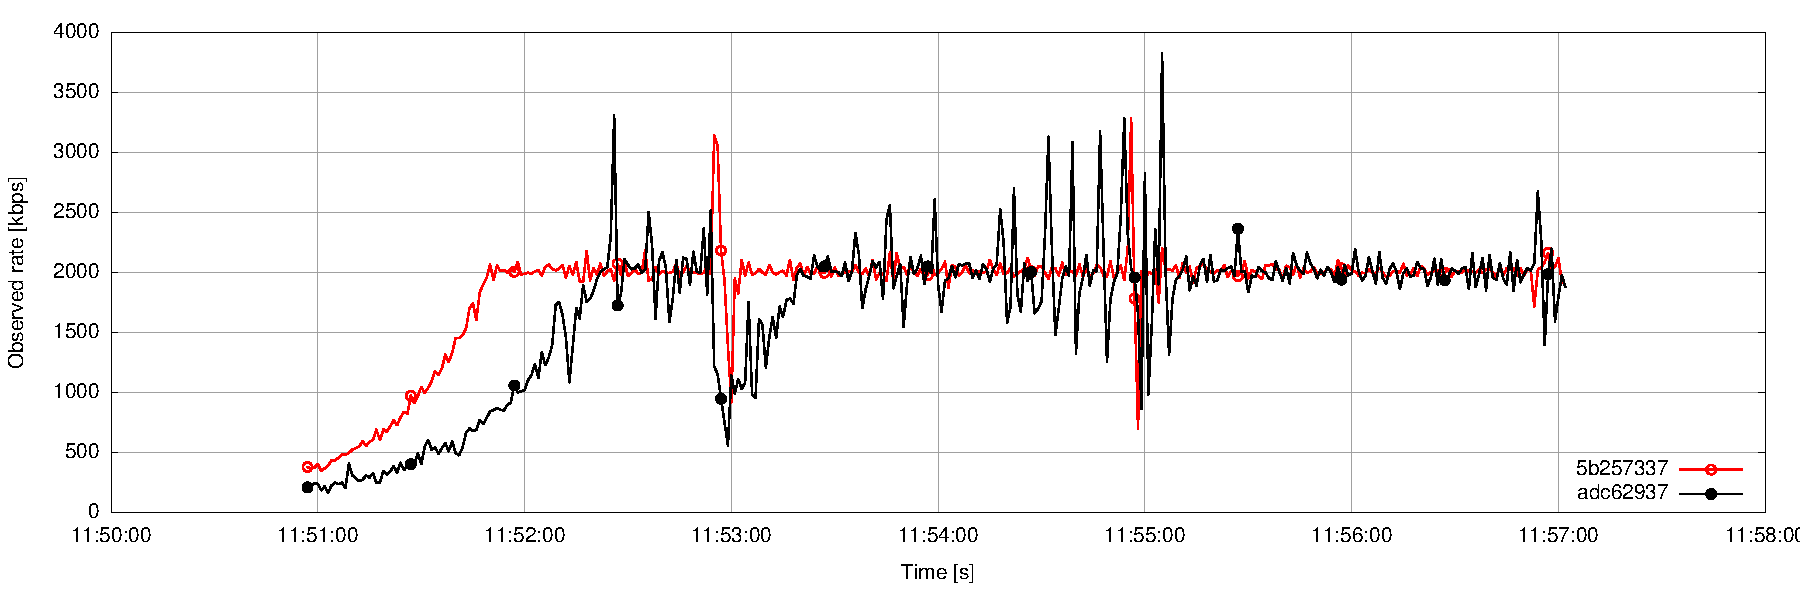
\includegraphics[width=1\textwidth]{./figures/onetooneWiFIStatsVideoStreams.pdf}
%      \caption[Point-to-point WebRTC input/output video throughput graph using Stats API over public WiFi]{Point-to-point WebRTC input/output video throughput graph using Stats API over public WiFi.}
%	\label{fig:onetooneWifiRTCVideoStreams}
%\end{figure}
%
%Figure~\ref{fig:onetooneWifiRTCVideoStreams} shows the two video streams captured from the same machine, one is outgoing the local video stream meanwhile the second stream is the incoming video stream from the other peer. We have built a flexible processing system that allows us to capture and analyze all the possible combinations of streams and metrics. The timing used for the capture is provided by the TimeStamp available on the RTCP. The average bandwidth used in this scenario of point-to-point call in a standard wireless network is around 2000 Kbps per video stream. Both figures are plotted from the same original call.

% \begin{figure}[h]
%  \centering
%    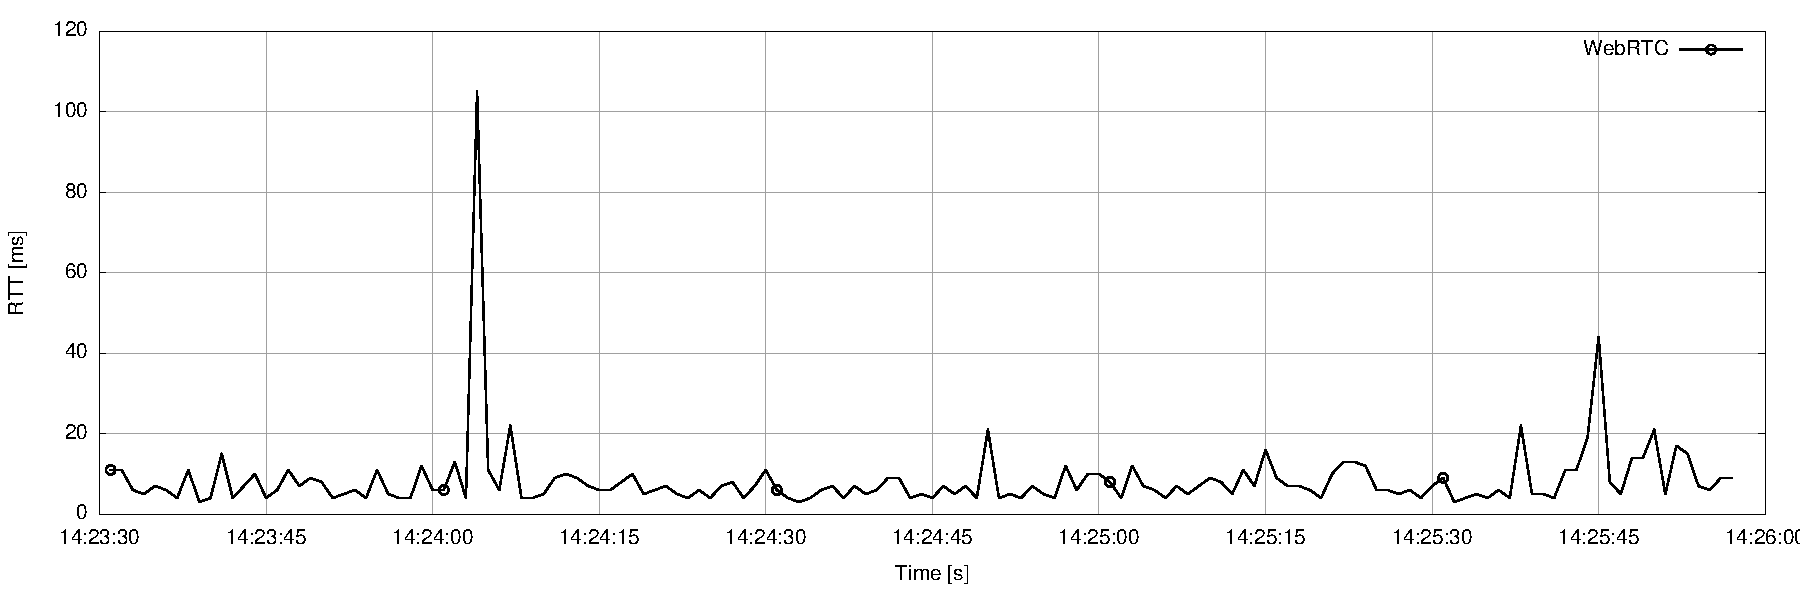
\includegraphics[width=1\textwidth]{./figures/p2prttexample.pdf}
%      \caption[Point-to-point WebRTC RTT measure using Stats API over public WiFi]{Point-to-point WebRTC RTT measure using Stats API over public WiFi.}
%	\label{fig:p2prttexample}
%\end{figure}

%Our Stats API also provides extra information such as RTT and loss rate, RTT should be provided natively by the WebRTC %method but it is possible to calculate it by using the DataChannel provided by the PeerConnection, we are using this %channel to send a UNIX TimeStamp object to the other peer and take it back, when the round trip is finished we compare it %with the actual millisecond and obtain the total RTT.

%Figure~\ref{fig:p2prttexample} represents the capture of a video call between two peers, if we are able to process the JavaScript forwarding function in an optimal way this would led to a precise RTT measurement hack without the need of Stats method.

\subsubsection{Analysis of tools}

Both tools will be measuring the same metrics but from different OS layers, this provides us some extra data to be considered in order to see how the our Stats API work and if it is possible to implement some extra features relying on that data for the WebRTC API.

Because of the period needed to measure the results it is possible to have strange behaviors when plotting the results as the information regarding to the next data period can be considered as the previous one. This is an accuracy problem that cannot be approached easily, when looking at the graph is important to see if both peaks (positive and negative) get compensated as this would mean that the data has not been allocated to the current period. This accuracy error is a problem that can be observed when comparing both {\it ConMon} and Stats API capture as the browser will take some time to process the stats and send them to the JavaScript method, this will led to some extra error.

Figure~\ref{fig:p2pincommingStatsConmonWifi} and~\ref{fig:p2poutgoingStatsConmonWifi} plot two video streams being captured from Stats API and {\it ConMon}.

\begin{figure}[h]
	\begin{minipage}{.5\textwidth}
		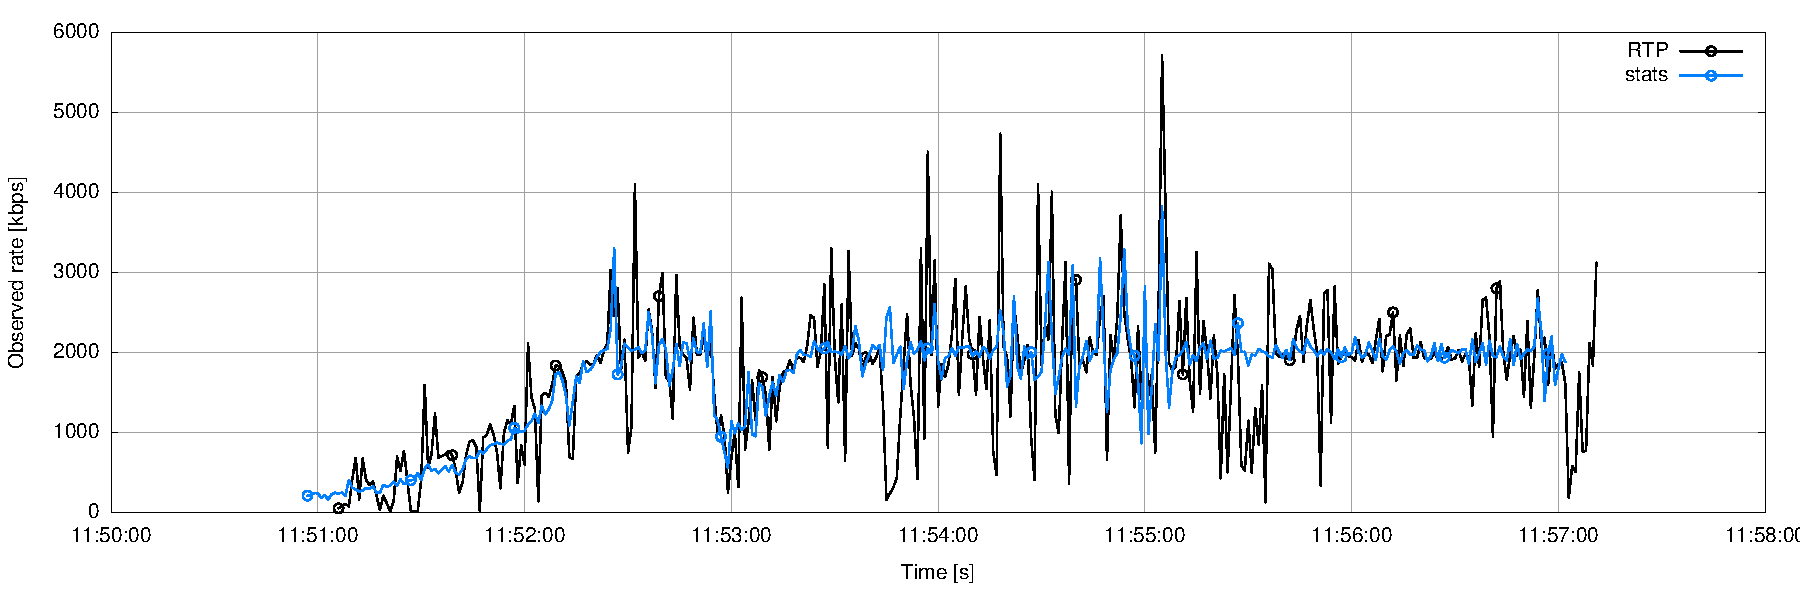
\includegraphics[width=1\textwidth]{./figures/p2pincommingStatsConmonWifi.pdf}
			\caption[P2P incoming video stream comparison between ConMon and Stats API over public WiFi]{P2P incoming video stream comparison between ConMon and Stats API over public WiFi.}
			\label{fig:p2pincommingStatsConmonWifi}
	 \end{minipage}
	 \begin{minipage}{.5\textwidth}
		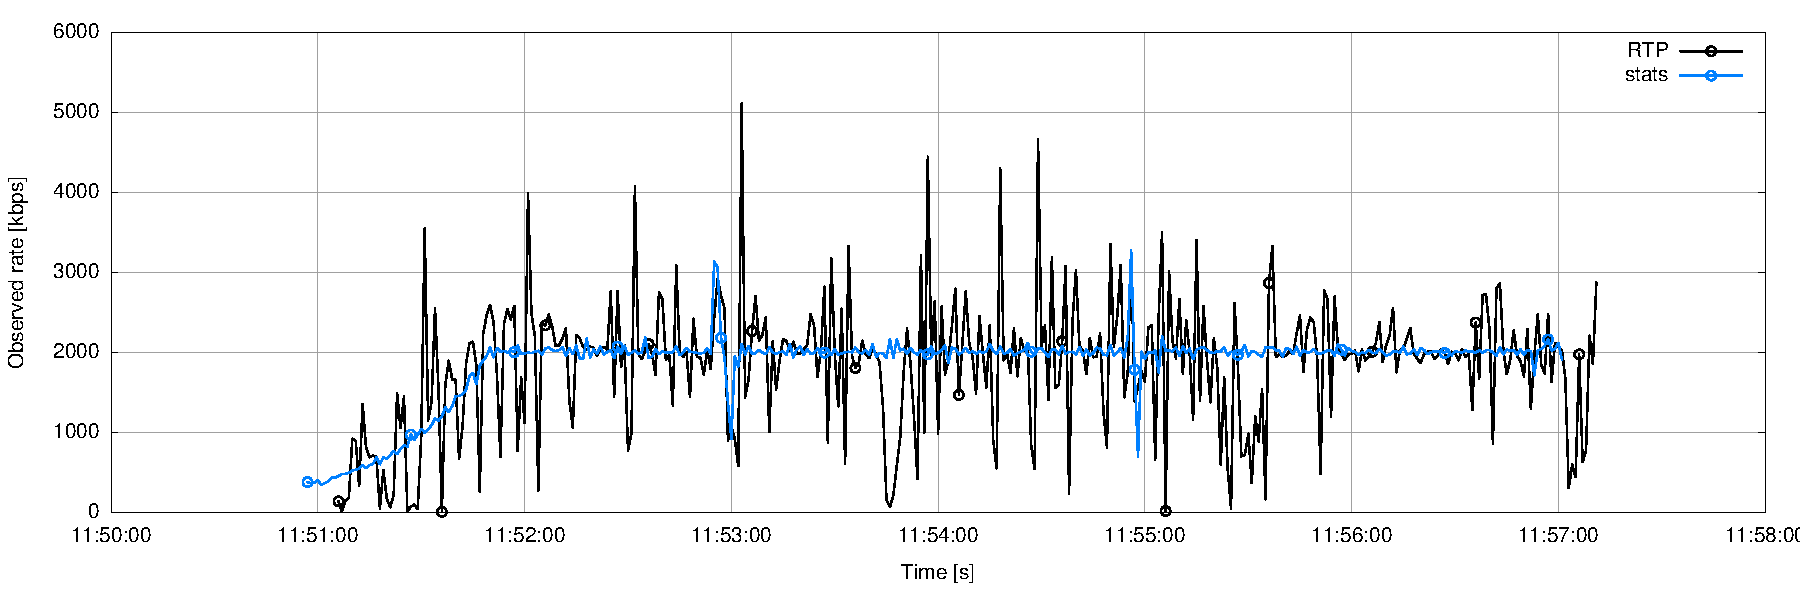
\includegraphics[width=1\textwidth]{./figures/p2poutgoingStatsConmonWifi.pdf}
			\caption[P2P outgoing video stream comparison between ConMon and Stats API over public WiFi]{P2P outgoing video stream comparison between ConMon and Stats API over public WiFi.}
			\label{fig:p2poutgoingStatsConmonWifi}
	 \end{minipage}
\end{figure}

Figure~\ref{fig:p2pincommingStatsConmonWifi} represents the incoming media stream from the other peer, this is why the throughput seems to be so unstable in some parts of the call, consider also that this test was performed using wireless connection without any network conditioner. In Figure~\ref{fig:p2poutgoingStatsConmonWifi} local stream is sent from the peer capturing with {\it ConMon} to the remote peer, the throughput captured using Stats API will be much more stable around the 2000 Kbps.

\subsection{Automated testing}

For our testing scenario we have considered two options, manual and automated testing. The first test environment does not give as much accuracy due to the impossibility to iterate the test many times for the same configuration, if the second option is available the results can be averaged with all the iterations leading to an accurate result.

When considering both, the media being sent becomes a problem as there should be rich enough to be able to replicate a real call scenario. Google Chrome provides a fake video that can be activated by adding {\it --use-fake-device-for-media-stream} parameter, this video though might be too simple for our purposes.

%\begin{figure}[h]
%	\begin{minipage}{.5\textwidth}
%		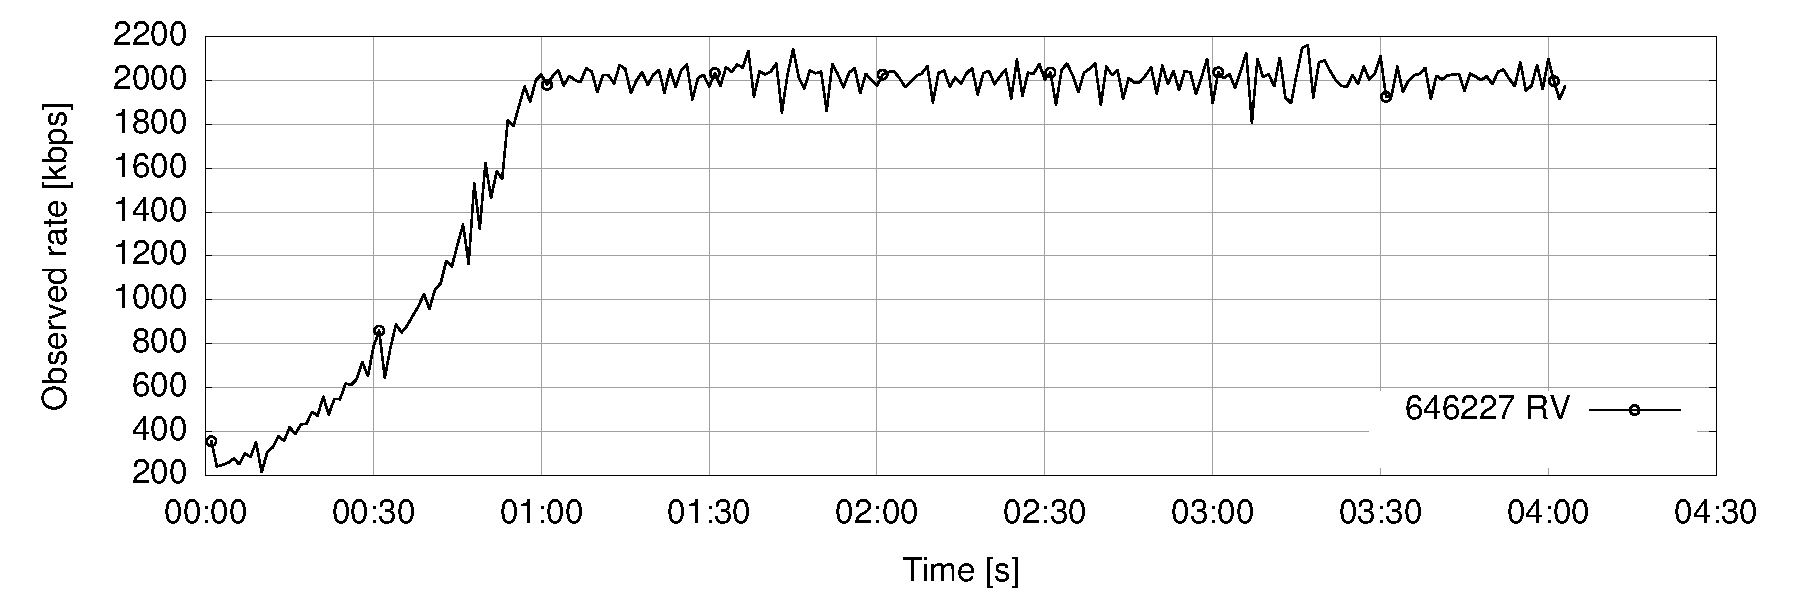
\includegraphics[width=1\textwidth]{./figures/realVideoChrome.pdf}
%			\caption[Video stream bandwidth between two peers using webcam]{Video call bandwidth between two peers using webcam.}
%			\label{fig:realVideoChrome}
%	 \end{minipage}
%	 \begin{minipage}{.5\textwidth}
%		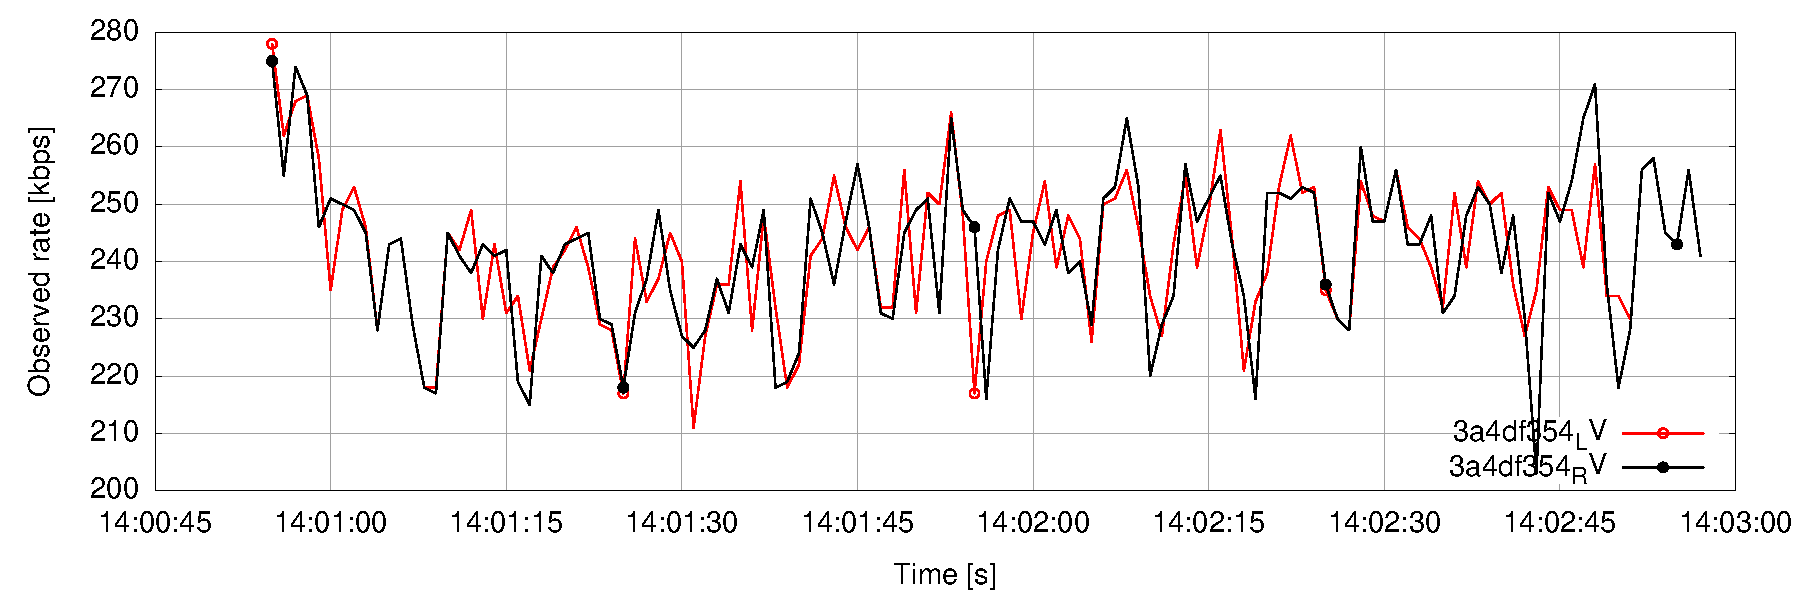
\includegraphics[width=1\textwidth]{./figures/automatedVideoChrome.pdf}
%			\caption[Video stream bandwidth between two peers using fake video]{Video stream bandwidth between two peers using fake video.}
%			\label{fig:automatedVideoChrome}
%	 \end{minipage}
%\end{figure}

 \begin{figure}[h]
  \centering
   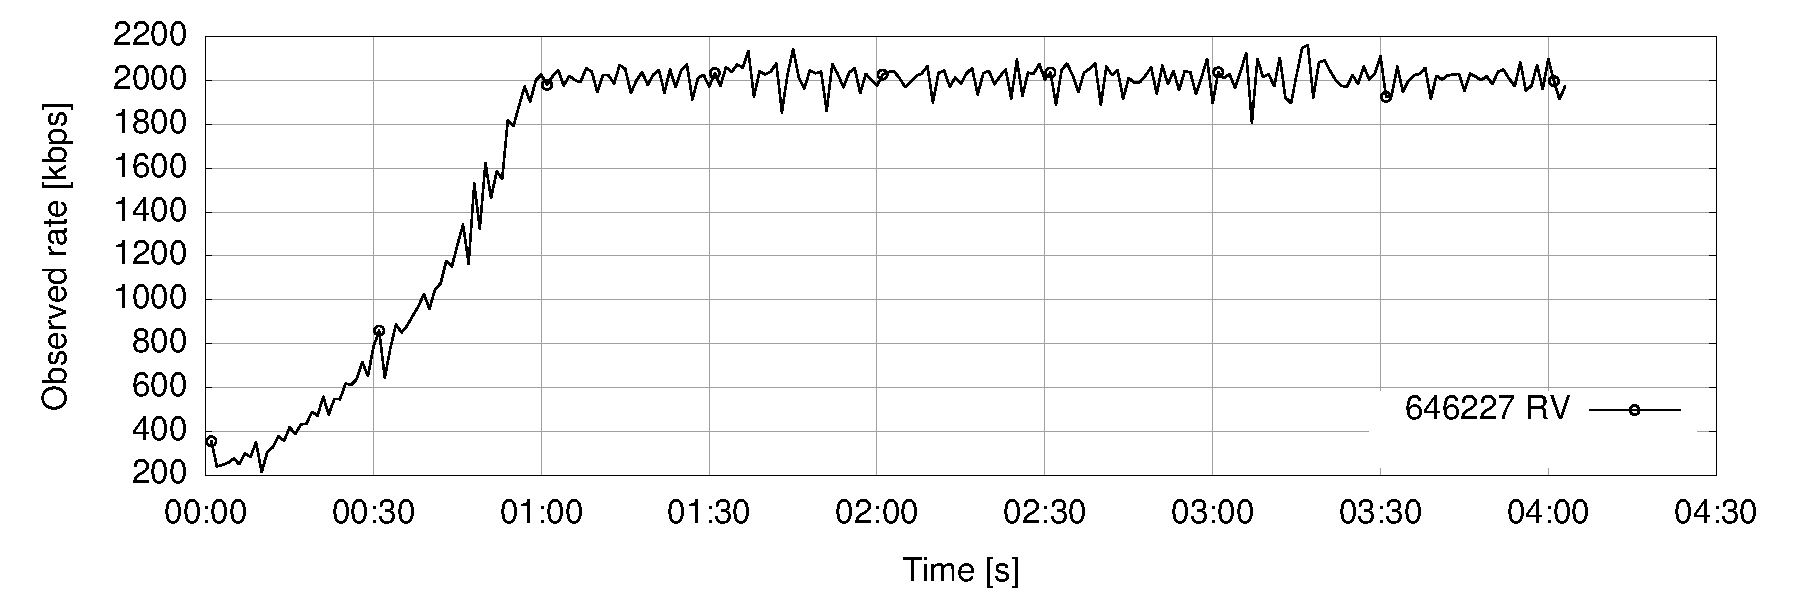
\includegraphics[width=1\textwidth]{./figures/realVideoChrome.pdf}
     \caption[Video stream bandwidth using webcam]{Video stream bandwidth using webcam input.}
	\label{fig:realVideoChrome}
%\end{figure}
 %\begin{figure}[h]
  \centering
	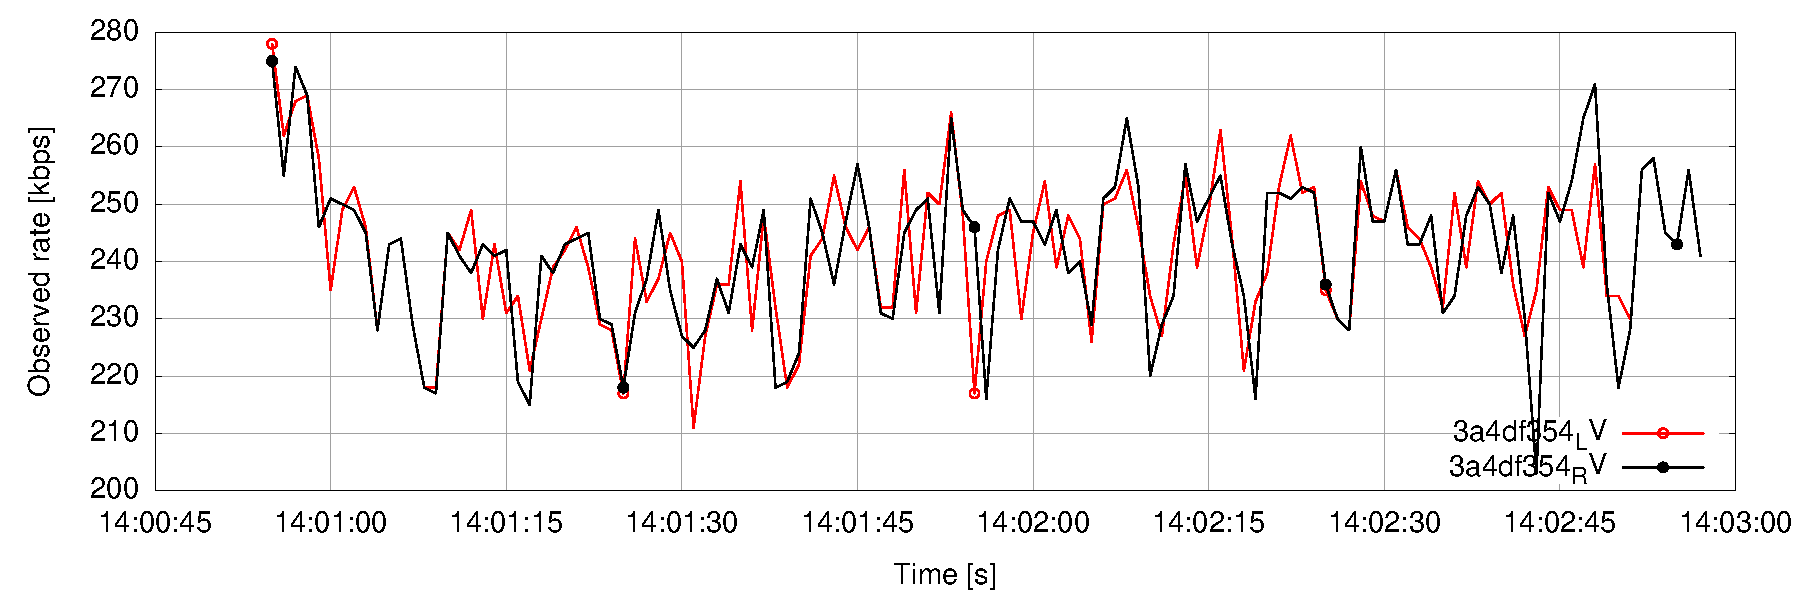
\includegraphics[width=1\textwidth]{./figures/automatedVideoChrome.pdf}
	\caption[Video stream bandwidth using Chrome default fake content]{Video stream bandwidth using Chrome default fake video input.}
	\label{fig:automatedVideoChrome}
\end{figure}

Figure~\ref{fig:realVideoChrome} represents the bandwidth that a real video call uses when sending the stream to the other peer, that capture shows the same stream from the origin an remote {\it StatsAPI} perspective. The bandwidth allocated goes up to 2000 Kbps. On the other hand, Figure~\ref{fig:automatedVideoChrome} represents the same call by using the built-in fake video on both clients, the bandwidth in this case drops to an average of 250 Kbps. Those figures represent the same stream identified with the SSRC that corresponds, input from receiver and output from origin, this representation helps us to identify any possible distortion on the link. Google Chrome uses a bitmap system to draw the figures and components to be rendered in the video tag, this means that the amount of encoding and bandwidth used is low compared to a real webcam.

To address this issue in the video streamed from our automated devices we have built a fake input device on the virtual machines, procedure is described in Appendix~\ref{sec:fakeVideo}.

 \begin{figure}[h]
  \centering
    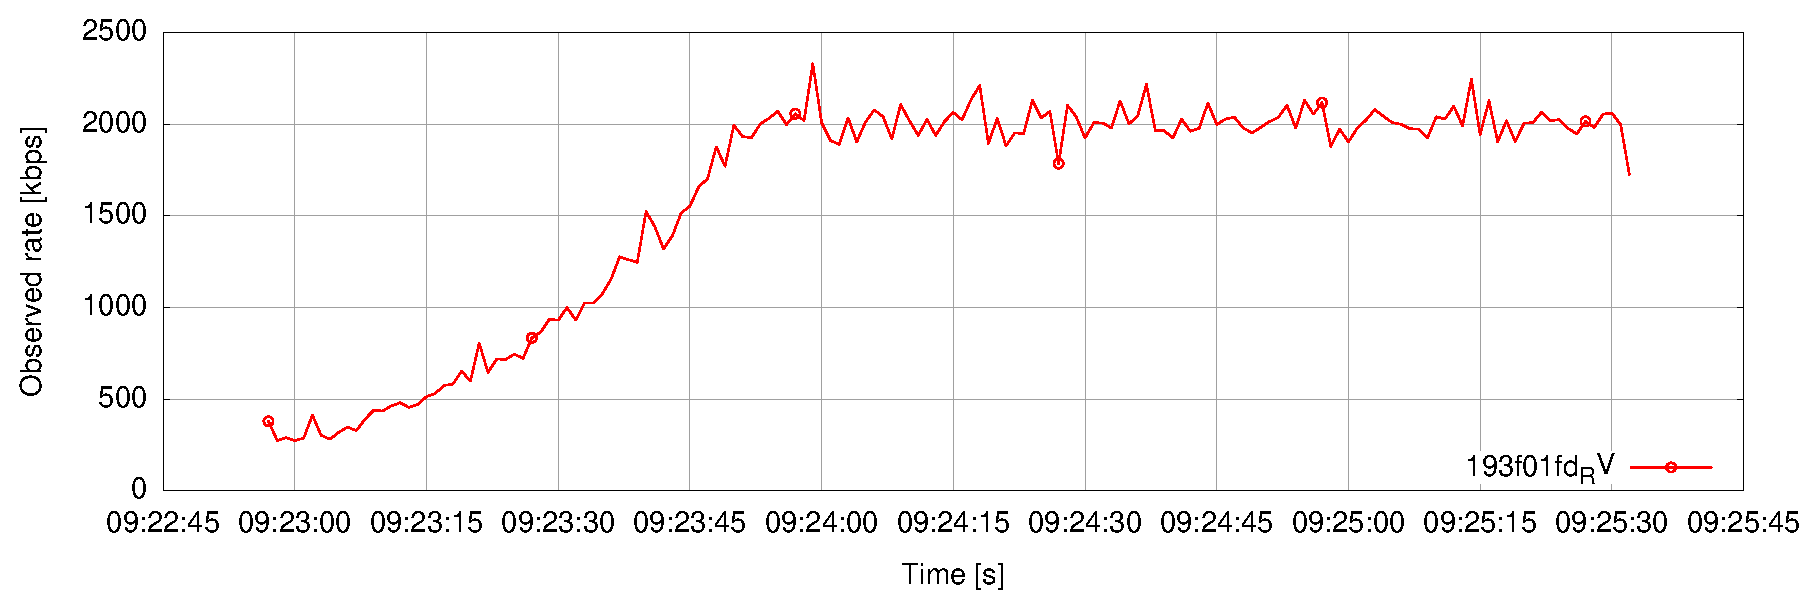
\includegraphics[width=1\textwidth]{./figures/testV4L2niklas.pdf}
      \caption[Video stream bandwidth using V4L2Loopback fake YUV file]{Video stream bandwidth using V4L2Loopback fake YUV file.}
	\label{fig:testV4L2niklas}
\end{figure}

Figure~\ref{fig:testV4L2niklas} shows the bandwidth of a video stream measured by our {\it Stats API} using an YUV video captured from a Logitech HD Pro C910 as source, resolution is 640x480 at a frame-rate of 30 fps. Results show an approximate average bandwidth of 2000 Kbps which is a realistic approach to a real webcam. This setup will allow us to run multiple tests without the need of a webcam.

\subsection{TURN Server}

Our TURN server is used to pipe all the media as a relay to apply the constraints required for the tests, this machine is a Ubuntu Server 12.04 LTS with a tuned kernel to perform better with {\it Dummynet}.

As TURN software we are using {\it Restund} which has been proven to be reliable for our needs, this open source STUN/TURN server works with{\it MySQL} database authentication~\cite{http://www.creytiv.com/restund.html}. We have modified the source in order to have a hardcoded password making it easier for our needs.

To do so, we need to modify {\it db.c} file before compiling. Method {\it restund\_get\_ha1} content should be replaced with the following line of code where XXX is username and YYY the password.

\begin{lstlisting}
md5_printf(ha1, "\%s:\%s:\%s", "XXX", "myrealm", "YYY");
\end{lstlisting}

This part is important as it allow us to set the constraints in a middle point without affecting the behavior of the WebRTC clients.

\subsubsection{Dummynet}

To check the performance of WebRTC we will need to modify the status of the network link. This is achieved using {\it Dummynet}, a command line network simulator that allow us to add bandwidth limitations, delays, packet losses and other distortions to the ongoing link.

{\it Dummynet} is an standard tool for some Linux distributions and OSX~\cite{dummynetTool}.

In order to get appropriate results with the constraints of the network we will have a machine acting as TURN for some tests, this machine will forward all the WebRTC traffic from one client to the other being transparent for both ends. The real goal of using TURN in WebRTC is to avoid and bypass some restrictive Firewalls that would block the connection, in our case, this works as a way to centralize the traffic flow through one path being able to be modified or tightened. From the performance perspective, when not adding any constraints to the TURN, the traffic and response is normal without the user noticing any difference.

Some problems arise when using {\it Dummynet} in our scenario, we will be using {\it VirtualBox} machines for some testing and to act as TURN, read Appendix~\ref{sec:dummynet} for more information about {\it Dummynet} configuration.

\subsection{Application Server}

Our application server will run the Node.js instance for the WebRTC signaling part, this machine runs Ubuntu with a domain specified as {\it dialogue.io}. This app is a group working application to allow people to chat and video call at the same time, we have modified it to build an specific instance for our tests, this instance will simply allow two users that access the page to automatically call each other and start running the JavaScript code with built-in {\it Stats API}

Most of this application is coded with JavaScript and use WebSocket protocol to carry the signaling messages.